%!BIB program = bibtex
\documentclass[9pt, twocolumn, twoside, lineno]{pnas-new}
% Use the lineno option to display guide line numbers if required.

% PNAS研究论文模板
\templatetype{pnasresearcharticle} % Choose template 
% {pnasresearcharticle} = Template for a two-column research article
% {pnasmathematics} %= Template for a one-column mathematics article
% {pnasinvited} %= Template for a PNAS invited submission
% \usepackage{cite}
\usepackage{url}	
% 文章标题:“流域尺度的水资源利用体系:过渡框架和发展困局”
\title{Regime transition identification for water governance of river basin}
\label{title}
% Use letters for affiliations, numbers to show equal authorship (if applicable) and to indicate the corresponding author
% 作者列表
\author[a, b]{Shuang Song}  % 宋爽,一作
\author[a, b, 1]{Shuai Wang}  % 王老师,通讯
\author[c, d]{Xutong Wu}  % 武旭同
\author[a, b]{Bojie Fu}  % 傅老师
\author[e]{Yongping Wei} % 尉老师

% 机构列表
\affil[a]{ % 北师大地表国重
	State Key Laboratory of Earth Surface Processes and Resource Ecology, 
	Faculty of Geographical Science, 
	Beijing Normal University, 
	Beijing 100875, 
	P.R. China
}
\affil[b]{ % 北师大地理学部
	Institute of Land Surface System and Sustainability, 
	Faculty of Geographical Science, 
	Beijing Normal University, 
	Beijing 100875, 
	P.R. China
}
\affil[c]{ % 北大城环
	College of Urban and Environmental Sciences, 
	Peking University, 
	Beijing 100871, 
	P.R. China
}
\affil[d]{ % 中科院生态中心
	State Key Laboratory of Urban and Regional Ecology, 
	Research Center for Eco-Environmental Sciences, 
	Chinese Academy of Sciences, 
	Beijing 100085, 
	P.R. China 
}
\affil[e]{ % 昆士兰大学
	School of Earth and Environmental Sciences, 
	The University of Queensland, 
	Brisbane 4067, 
	Australia
}

% Please give the surname of the lead author for the running footer
% 领衔作者
\leadauthor{Song} 

% Please add a significance statement to explain the relevance of your work
% PNAS特有的“Significance陈述”,用不超过120个字来说明研究的意义和亮点
\significancestatement{
	% Authors must submit a 120-word maximum statement about the significance of their research paper written at a level understandable to an undergraduate educated scientist outside their field of speciality. The primary goal of the significance statement is to explain the relevance of the work in broad context to a broad readership. The significance statement appears in the paper itself and is required for all research papers.
	Water, a key resource to support the sustainable development of human societies, whose natural cycle has been modified by growing socio-economic processes. We propose a new method with an integrated index to detect water utilization regimes and applying it to the Yellow River Basin, a typical overexploited basin in China. After sketching changes of relationships between social development and water utilization within the Yellow River Basin, we summarized a general transition framework. By predicting widespread development dilemmas, it can be a useful guideline for basins all around the world in their sustainable developing trajectories. 
}

% Please include corresponding author, author contribution and author declaration information
\authorcontributions{ % 作者的相应贡献
	Shuai Wang and Bojie Fu designed this research,
	Shuang Song performed the research and analysed data,
	Shuang Song, Xutong Wu wrote the paper.
}
\authordeclaration{ % 利益冲突陈述
	The authors declare no competing interests.
}

% 如果有共同一作的情况,则uncomment下面这行代码的注释
%\equalauthors{\textsuperscript{1}A.O.(Author One) contributed equally to this work with A.T. (Author Two) (remove if not applicable).}

% 通讯作者信息
\correspondingauthor{\textsuperscript{1}To whom correspondence should be addressed. E-mail: shuaiwang@bnu.edu.cn}

% 关键词,三到五个
% At least three keywords are required at submission. Please provide three to five keywords, separated by the pipe symbol.
\keywords{Regime shifts $|$ Sustainability $|$ Instructional fit $|$ Water governance challenges $|$ River basins} 

%tag 摘要
\begin{abstract}
	\label{abstract}
	% For water utilization as blood that sustains social developments, humans have harnessed basins, modified river cycles and triggered a range of regime shifts all around the world.
	For sustaining socio-economic development, human have harnessed large rivers and triggered a range of regime shifts at a basin scale all around the world. 
	Detecting these abrupt reorganizations of structure and function is critical to successful future river basin management. 
	Here, considering three main dimensions of water utilization (stress, priority and configuration), we develop an Integrated Water Resources Utilization (IWRU) Index at a basin scale to indicate regime shifts. 
	By applying this index to the Yellow River Basin, China, it suggests that there were two regime shifts over half a century, whose drivers were economic growths, managements and efficiency improvement.
	Differ from previous onefold descriptions, IWRU captures various considerations intertwined in water utilization, based on which we proposed a transition framework in interpreting associated changes.
	By identifying and predicting widespread dilemmas in transition of water utilization, this framework can be a useful guideline for big river basins to develop in a coordinated way.
\end{abstract}


\dates{This manuscript was compiled on \today}
\doi{\url{www.pnas.org/cgi/doi/10.1073/pnas.XXXXXXXXXX}}


\begin{document}

\maketitle
\thispagestyle{firststyle}
\ifthenelse{\boolean{shortarticle}}{\ifthenelse{\boolean{singlecolumn}}{\abscontentformatted}{\abscontent}}{}
% If your first paragraph (i.e. with the \dropcap) contains a list environment (quote, quotation, theorem, definition, enumerate, itemize...), the line after the list may have some extra indentation. If this is the case, add \parshape=0 to the end of the list environment.

\label{introduction}
% tag 引言第一段
% 水资源在人类世的重要性,是支持人类社会发展的基础。
\dropcap{W}ater, at “the centre of the planetary drama of the Anthropocene”, is not only essential for myriad Earth system processes, but also supporting development of human societies in various aspects. 
% TODO 这里增加三篇“大文章”参引
% 但同时, 人类的改造也深刻影响了自然水循环过程, 相关变化可能影响人水系统功能的不利转变,并带来发展困局。
However, human's modification has profoundly influenced the water cycle, which may lead adverse changes to functions of human-water systems, resulting in development dilemmas \cite{gleesonIlluminatingWaterCycle2020,cummingLinkingEconomicGrowth2018}.
% TODO 这里增加参考文献,人类对水循环的改造 
% 大河流域常是经济和文明发展的中心,同时也是面临人类世压力挑战的主要地区,亟需综合水资源治理以实现可持续发展。
Facing major challenges in the Anthropocene, many of the world's big river basins, also hot spots of economy and civilization, urgently need integrated water resources management toward sustainability \cite{bestAnthropogenicStressesWorld2019}. 
% 因此理解人类社会发展与水资源利用的复杂关系,对此有帮助。
Since it requires deep understanding of the complex relationships between human societies and water resources utilization, sketching their transitions provides underlying supports for developing in a coordinated and sustainable way at a basin scales.

% tag 引言第二段
% Regime 和 Regime shift 的定义。
Regime is a stable state of system’s structure and function, whose large and persistent changes may lead to substantive impacts on the outcomes of system with widespread cascading effects, defined as regime shifts \cite{rochaCascadingRegimeShifts2018,schefferCatastrophicRegimeShifts2003, schefferCatastrophicShiftsEcosystems2001}.
% 人水系统中的水资源功能
Water have several key functions within a human-water system, the most important of which is sustaining the development of human societies through water utilization. 
% 水资源利用 regime shift
However, interplayed human interference, such as water withdrawal, dam constructions and water managements have significantly changed water functions and induced changes in water use
\cite{falkenmarkUnderstandingWaterResilience2019}.
% 稳态转换随着社会发展增加
These gradual or abrupt changes triggered regime shifts as societies' development strengthen their interlinks to water utilization with increased dependences.
% TODO 这里需要安排参考文献,稳态转换的触发方式,随着社会发展更多
% Regime 过渡性的存在
As a result, most large river basins had gone through phases of accelerated exploitation, over-exploitation, and integrated management, for which it is a reasonable assumption that there is a general transition pattern in water utilization. 
% TODO 这里需要安排参考文献,大河流域的发展历程
% 因此,识别水资源利用的稳态变化,并从中寻找一般性的发展模式,有助于理解流域存在的问题
Identifying the regime shifts in water utilization and sketching a general pattern, therefore, can help to understand and predict developing trajectories of basins, which are crucial for integrated management and coordinated development towards sustainability.

% 这里删掉的部分
% % 过渡性有助于理解流域存在的问题
% Sketching the transition of water utilization regimes, therefore, can help to understand and predict developing trajectories of basins, which are crucial for integrated management and coordinated development towards sustainability.
% % 对过渡性的研究还很少
% Despite pervasiveness, there is still lacking of effective method to distinguish the water utilization regimes and detect regime shifts, with much fewer attempts to develop theoretical models to explain their transitions as well. 

% Tag 引言第三段
% 前人已经从不同维度刻画了人水关系.
Features of water utilization has been depicted and studied from various intertwined perspectives.
% 首先,因为水资源的稀缺性和全球用水量的增加,受到最广泛关注的是人类社会面临的水资源压力。
Firstly, water stresses are of increasing importance and concerns.
Greater water utilization stresses had become a major constraint to development, because of significant increment in water withdrawals and larger shares of inflexible water use, while store of water resource in reservoirs are helpful to relief of
\cite{postelHumanAppropriationRenewable1996, greveGlobalAssessmentWater2018, qinFlexibilityIntensityGlobal2019}.
% 其次,随着工业迅猛发展和生态建设的需要,社会对水资源的利用的倾向性也发生了转变。
Secondly, as the priority of water utilization changed with the need of development. 
There are noticeable growths in economy profits of industry or services and their priority in water use, leading potential conflicts between different sectors
\cite{liuWaterScarcityAssessments2017, florkeWaterCompetitionCities2018}.
% 最后,由于水的可用性本质上是区域问题,水资源利用的格局也很重要
Thirdly, since development are inherently regional concerns, where heterogeneous regions attempt to develop themselves by economically competitive sectors, configuration of water resources also plays as an important aspect.
% 全球总的取水量很少,但缺水地区很多
% As a result, while only 10\% of available water is withdrawn on global average, about 30\% of population settles in severe water-stressed regions for higher level of development
% \cite{wadaWedgeApproachWater2014, okiGlobalHydrologicalCycles2006}.
% 总的来说,上述三个维度试图解答与水资源利用有关的三个重要问题 “还有多少水资源可以利用”,“把水资源用在什么”
Taken together, existing researches have evaluated the three dimensions of water resource utilization regarding a series of crucial questions: ``How much water resources?'', ``How to use them?'' and ``Used for whom or in where?''.
% 将三种视角结合,就是“水资源利用体系”。
However, these dimensions haven't been well integrated by quantitative methods, and a coherent interpret of regime shifts regard to social development and water utilization is needed.


% tag 引言最后一段
% 这里我们整合了三个方向,提出了描绘流域人水关系的指数
Here, by integrating three above mentioned dimensions of water utilization, we develop an Integrated Water Resources Utilization (IWRU) Index at a basin scale to give a sketch of relationships between human societies and their water utilization (Figure~\ref{fig:framework}).
% 使用案例研究
Then, by applying this index to the Yellow River Basin, China, we analysed water utilization regimes shifts and their drivers in this typical basin of anthropogenic impacts.
% 最后总结出一般性框架
Finally, we proposed a transition phases framework of development echoing to the regime shifts, which can be a useful guideline for basins to predict dilemmas in water utilization and to develop in a coordinated way.


\begin{figure*}%[htbp]
	\centering
	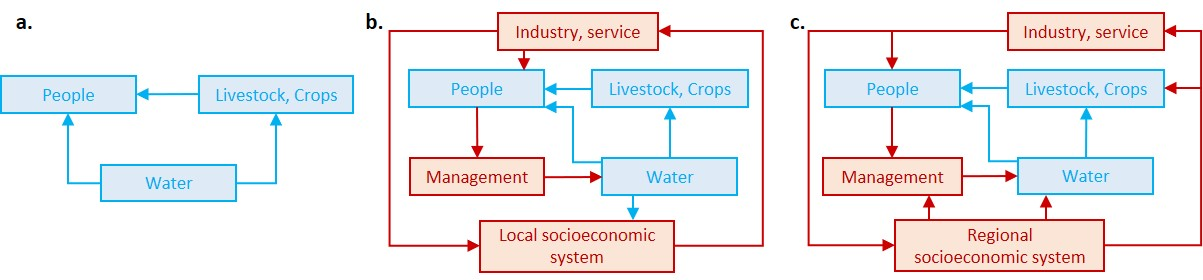
\includegraphics[width=0.8\linewidth]{../../figures/main/framework.jpg}
	\caption{
		A schematic diagram for understanding the changing relationship between social development and water utilization.
		% 图A是水资源利用的三个维度。每个维度都有两个极点(红色字表示),指示水资源利用在该轴上的两个变化方向。
		\textbf{A,} three dimensions (stress, priority and configuration) of water resources utilization. Each dimension has two poles (denoted in red) which indicates the two potential directions of water resources utilization changes along that axis. (1) Stress of water utilization shifts between scarcity of water resources and abundance of water resources, which means there is shortage of water supply or not. (2) Priority of water utilization can move between a provisioning part or a non-provisioning one, indicating how much water were used in food supporting to human societies. (3) configuration can move between balanced or lopsided, when allocation of water resources between different sectors or regions changed. We presume that water utilization regimes equally weighted by these basic dimensions, whose combination can highly relate to basin development. 
		% 图B是将三个维度结合后的变化情况。因上述三个维度随着社会发展而不断变化,其组合的水资源利用状态也不同。这个过程中当突变发生时,可能标志着水资源利用发生了稳态转换,因此我们需要一个指标来监测其变化。
		\textbf{B,} the changes after combining the three dimensions. Because the above three dimensions are changing with the development of society, their combined water resource utilization status is also different. When abrupt transitions occur during this process, they may indicate a regime shift in water utilization, so we need an indicator to monitor this change.
	}
	\label{fig:framework}
\end{figure*}


\section*{Results}
\subsection*{Water utilization regimes}

\begin{figure}[ht!]
	\centering
	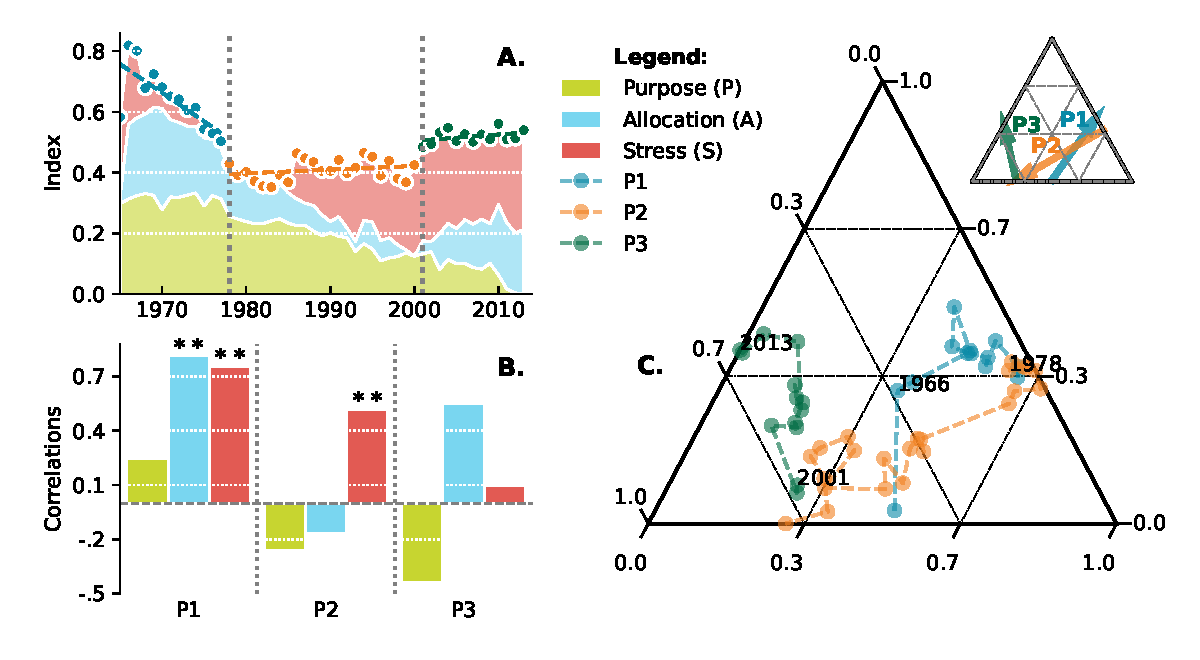
\includegraphics[width=\linewidth]{../../figures/main/index.pdf}
	\caption{Changes of the IWRU index. 
	\textbf{A,} Change points detection. With change points in 1978 and 1994, the IWRU have three periods in changing trend.
	\textbf{B,} Changing slopes of each period.
	\textbf{C,} Contributions of each dimension to the changes of IWRU within three periods. Stress, priority and configuration are the main positive contributor of P1, P2 and P3, respectively.
	}
	\label{fig:IWRU}
\end{figure}

% 这一节主要展示IWRU的变化趋势和WUR的划分
With two significant points, the changing trend of IWRU index are detected into three periods (Figure~\ref{fig:IWRU}A). 
Not only the slope of changes are various within each period, changes are also mainly contributed by different dimensions (Figure~\ref{fig:IWRU}B and Figure~\ref{fig:IWRU}C).
% 第一阶段
In the first period (P1, 1965-1978), the IWRU index had a rapidly increasing and the lightening of water stresses made the most striking positive contribution (131\%), while priority and configuration of the water utilization had slight negative contribution (-11\% and -20\%).
% 第二阶段
In the second period (P2, 1979-1994), though contributions of priority and configuration turned into positive, the IWRU index experienced a drop because of stresses on water resource playing a larger negative role (-188\% dropped than P1). 
% 第三阶段
However, as the further increasing of positive contributions of priority (75\%) and configuration (84\%), and decreases of water stresses in negative contribution (-59\%) in the third period (P3, 1995-2013), a positive growth of the IWRU returned.

\begin{figure}[!htbp]
	\centering
	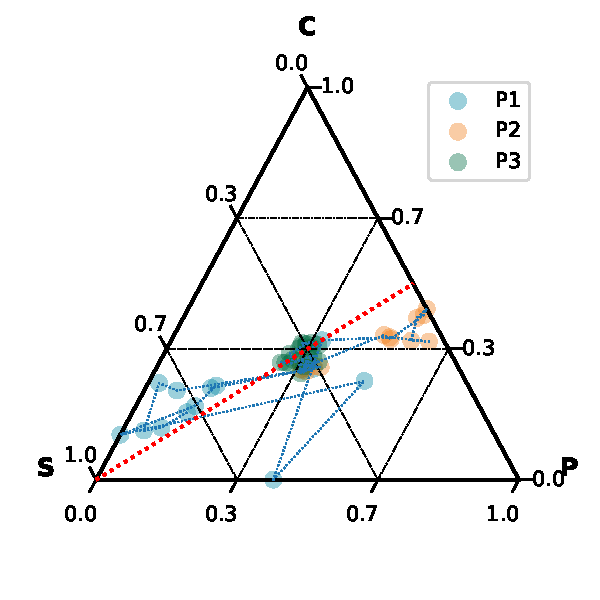
\includegraphics[width=0.9\linewidth]{../../figures/main/phases.pdf}
	\caption{Combination of contributions regards three dimensions in different periods (S: stresses; P: priority; C: configuration). The closer a point to an angle of the triangle, greater the proportion of the contribution of this dimension.
	The red indicator line in this ternary plot denotes 1:1 contributions between priority (P) and configuration (C). When the points are bellow this line, the contribution ratio of configuration is lower than that of priority, and vice versa.}
	% 由于阶段一的点位于该线上方,L的净贡献比例多于P,而第二阶段的点则恰好相反。
	\label{fig:phases}
\end{figure}

% 总而言之,每个阶段都由水资源利用的不同维度提供最大的正向作用
Taken together, each period has the unique most striking positive contributor to IWRU, and overall features of three dimensions in different periods are shown in Figure~\ref{fig:phases}.
% 第一阶段到第二阶段
At the very beginning (1965) and throughout the whole P1, water utilization regime dominated by high stresses. After then, it experienced a shift to low stresses since 1978, with a change in the proportion of contributions between priority and configuration, too.
% 第三阶段集中
Finally, the contribution of three dimensions were much similar in P3 (32.91\%, 31.87\% and 35.21\% for priority, configuration and stress respectively), making the points highly concentrated at the centre of the ternary diagram in that period.


% %tag 结果2
% \subsection*{Differences between water utilization regimes}
% % 在不同的维度下各阶段进行对比,可以发现不同的水资源利用体系间存在明显差异。
% The differences between the water utilization regimes are reflected in changes of all three dimensions.

% % 从阶段一到阶段二,水资源压力的变化最为明显
% Moving from the regime in P1 to P2, the most striking change is the reversal of the trend in water utilization stress(Figure~\ref{fig:dimensions}A), which is determined by a combination of scarcity, flexibility and variability (Figure~\ref{fig:dimensions}D and \textit{SI Appendix} Method S4).   
% % 1. 水资源丰富,耗水量少且灵活用水
% In the P1, natural surface water resources were rather abundant with fewer water consumptions (\textit{SI Appendix} Fig. S3) and most of which were flexible water utilization (\textit{SI Appendix} Fig. S4). During the P1 and even P2, however, water consumption increases rapidly and natural surface water resources decreases at the same time, making water increasingly scarce. Opposite effect to that, numerous reservoirs built reduced the variability of water resources by boosting storage capacities, but there are much fewer reservoirs built in P2 (\textit{SI Appendix} Fig. S5). As a result, water utilization stress decreases during P1, but begins to rise rapidly in P2.

% % 另一方面,P2-P3,持续变化的水资源利用倾向与格局
% On the other hand, as the most positive contributors to the IWRU index in P2 and P3 separately, priority (Figure~\ref{fig:dimensions}B) and configuration (Figure~\ref{fig:dimensions}C) of water utilization were keeping to enlarge their impacts. 
% % 首先是用水比例的变化
% Representing priority of water utilization, increasing non-provisioning share of water utilization were mainly contributed by larger industrial water consumptions and minor total water uses, while their influences are weakening (Figure~\ref{fig:dimensions}E).
% % 再讨论用水格局的变化
% However, configuration of water utilization, whose contributions to the IWRU are increasing, were mainly benefited from decreasing differences in the amount of water resources used, both intersectoral and regional (Figure~\ref{fig:dimensions}F).


% tag 结果3
\subsection*{Drivers of water utilization regime shifts}

\begin{figure}[th!]
	\centering
	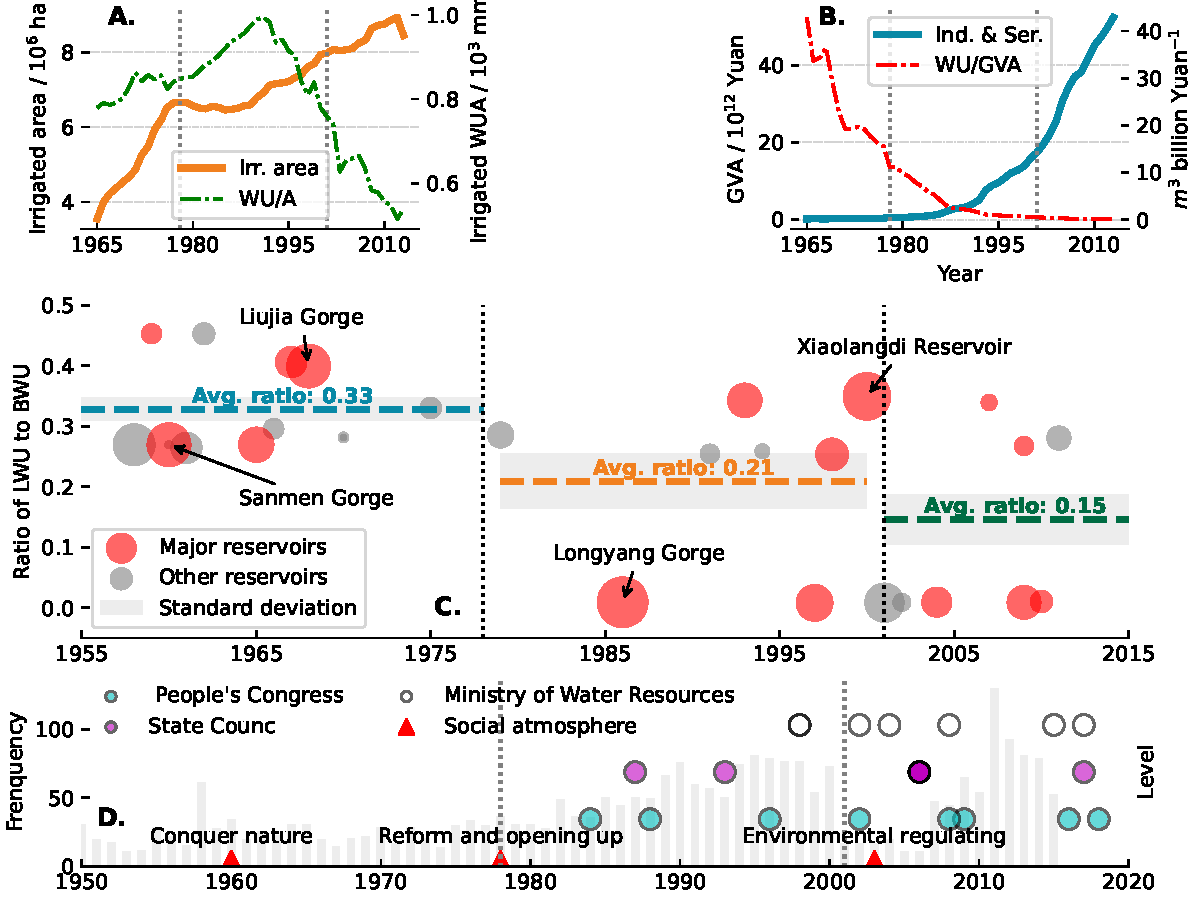
\includegraphics[width=\linewidth]{../../figures/main/causes.pdf}
	\caption{
		Drivers of water utilization regime shifts: economy growths, efficiency changes, and management practices.
		\textbf{A.} Changes of total irrigated area, and water consumptions in per unit of area (\textit{SI Method} S2).
		\textbf{B.} Changes of gross values added (GVA) of industry and services, and their water use density (WUI) respectively (\textit{SI Appendix} Method S2).
		\textbf{C.} Completed time of each new reservoir and their located regions' water use percentages in basin's total water use (WU), at that time. Red ones denote hub reservoirs in the basin, which plays a role in basinal integrated water management. Size of the points indicates their magnitude of water storage capacities. Some important or special reservoirs' name denoted: (1) Xiaolangdi reservoir and Sanmen Reservoir were constructed mainly responsible for managing sediments of the Yellow River. (2) Liujia Gorge, Longyang Gorge, were constructed mainly responsible for managing water flood discharge and storage. These marked reservoirs, therefore are significant for the entire basin, far crucial than regional development.
	}
	\label{fig:Causes}
\end{figure}

% 经济总量提升导致资源耗竭的加速。
Firstly, the expansion of irrigated area and the economic growth of industry and services are keys to the changes in the priority of water utilization between P1 and P2 (Figure\ref{fig:Causes}A). During the P1, irrigated agricultural area in the Yellow River basin expanded rapidly at a rate of $0.25*10^6 ha/yr$, and irrigation water was the dominant utilization way ($81.56\%$ of the total water use in 1965, and $83.17\%$ in 1978, see \textit{SI Appendix} Fig. S7). Entering P2, however, while the expansion of irrigated area stalled, industry and services gradually took off and took up more water resources (Figure\ref{fig:Causes} B), leading to $8\%$ reduction of proportion of irrigation water (\textit{SI Appendix} S7).

% 用水关系的变化
Secondly, efficiency of water utilization changed from the P2 to the P3.
While irrigated area resumed expansion again in the P3 whose water consumptions were still dominant (Figure\ref{fig:Causes}A), both industry, urban services were boosting their gross added values (GVA) (Figure~\ref{fig:Causes}B). 
However, the water use density (WUI) of them experienced significant declines and reached the lowest points (Figure~\ref{fig:Causes}A and Figure~\ref{fig:Causes}B).
It means, water utilization ways  have changed, along with technological solutions and a range of water conservation practices (\textit{SI Appendix} Fig. S8). As a result, the differences between the sectors of water use reduced while the total water consumption remains stable, during the P3 (\textit{SI Appendix} Fig. S7).

% 不断变化的管理模式。
Finally, changing water management practice contributed throughout all three periods. 
According to the location, we calculate the ratios of regional and basinal water use for each reservoir.
In the P1, most of the reservoirs are built in regions with high water demands, as ratios are significantly higher (Figure~\ref{fig:Causes}C, p<0.01). 
In the P2, the number of new reservoirs decreases significantly with little increment of total storage capacities (\textit{SI Appendix} Fig. S6). 
Entering the P3, however, the number of new reservoirs are even much higher than that in the P1, and most of them were built in regions with lower ratio of regional water use (Figure~\ref{fig:Causes}C and \textit{SI Appendix} Fig. S6).

% tag 讨论
\section*{Discussion}
\label{Discussion}
% Water governance challenges along transition regimes

% Implications and future directions
\subsection*{Shifted water utilization regimes with the development of society}
% 我们发明的指数能将三个维度的变化捕捉到。
The IWRU index captures the complex human-water feedbacks that links social development and water resources utilization from three dimensions (stress, priority and configuration). 
% 我们为的研究结果表明,黄河流域能被识别为三个明显的稳态
Our results show that three distinct regimes of water utilization within YRB, which have been driven by different causes regarding the three above dimensions.
% 在第一个稳态时期(即P1: before 1978),黄河流域农业的GDP贡献曾达到,超过经济效率通常更高的工业和服务业。
At the beginning of P1, the contribution of agriculture in the YRB to GDP was nearly a half (46\% in 1965), much higher than that of industry or services (33\% and 26\% in 1965, respectively see \textit{SI Appendix} fig. S9). 
% 考虑到彼时下游的工业用水尚未从黄河取水,且按省估计的夸张,这个数字仍远远低估了黄河流域的社会发展对农业的依赖。
Given that downstream industrial water had not depended on Yellow River yet, and the provincial estimates are exaggerated in industrial or services GDP (\textit{SI Appendix} Methods S3), this figure still greatly understates the dependence on agriculture for social development.
% 因此那时候,黄河流域主要管理组织黄河水利委员会()的主要工作之一是成立水利机构从事水利建设,而新建设的水库也多分布于高需水的区域。
At that time, one of the main tasks of the Yellow River Conservancy Commission (YRCC), therefore, was to set up agencies for water infrastructure \cite{yellowriverarchivesOrganizationalHistoryYellow2004}, and the new reservoirs were mostly distributed in regions with high water demands (Figure~\ref{fig:Causes} C). 
% 结果是,该稳态的主要特征表现为灌溉用水的迅速扩张,以支持农业发展。
As a result, this regime is characterized by a rapid expansion of irrigation water to support development of agriculture.

% 但因水资源危机的到来,上一制度与扩张性的农业发展随之结束,此时黄河耗水量已占天然径流量的约77%。
% 1972年,黄河首次断流19天,断流长度达310km,并连续多年断流。
The regime nearly came to an end with the water resource crisis, as the water consumption of the Yellow River had accounted for about 80\% of the natural runoff. As the most obvious performance, the Yellow River was dried up for several times since 1972 (\textit{SI Appendix} Fig. S10). 
% 来到1978年的制度时,黄委会领导改组,并接到水利部的批示,要求恢复和加强水文和流域管理相关的工作,
During the regime since 1978, the YRCC undergone a reorganization and received instructions from the Ministry of Water Resources (called Ministry of Water Resources and Electric Power then) to resume and strengthen work related to hydrology and basin management in YRB.
% 自此,稳态农业的扩张趋势得到了遏制(图causes),大部分流域尺度及以上的法律规章从此开始逐步推行,并在1987年提出了影响深远的“87分水方案”,为流域内各省份限定了可引水量
Since then, the expansion trend of agriculture has been constrained (Figure~\ref{fig:Causes}A), while the importance of industry began to increase with the Reform and Opening-up policy. In addition, most laws and regulations have been successively implemented (\textit{SI Appendix} Table 2). For an example, the far-reaching “87 Water Diversion Scheme”, which was put forward in 1987, limited the amount of water withdraw for each province as a constant in the YRB.

% 下一次稳态转换直到1993年左右才由用水效率的显著提升而带来。
The next regime shift was not occurred until a significant increase in water use efficiency since about 1993. 
% 此时在经历了十余年发展后,经济的重心已经倾向了工业和服务业,农业在GDP中的比重此时只占23%。
After more than a decade of development, the focus of economy had shifted to industry and services whose contribution of GDP in YRB are 45\% and 31\%, while agriculture accounting for only 23\% (\textit{SI Appendix} Fig. S9).
% 经济增长的同时,工业用水需求也迅速增加,两者推动了用水效率低下的农业实施节水改革。
A rapid increase in industrial demand for water has been accompanied by economic growth, which had led to water-saving reforms in inefficient agriculture. As a result, water use efficiency improved significantly in both agriculture and industry during the third regime (Figure~\ref{fig:Causes}A and Figure~\ref{fig:Causes}B), with engineered water-efficient irrigation reaching nearly half (48.6\%) of the total irrigated area (\textit{SI Appendix} Fig. S7), allowing the average water consumption per unit of irrigated area to drop about tenfold (Figure~\ref{fig:Causes}A).

In short, agricultural expansion, industries and services expansion, water resources management, as well as scientific and technological progress and water use efficiency improvement are intertwined in human-water system. They have driven the YRB to change regimes twice between 1965 and 2013, which can be interpreted as a transition process along with social development.

\subsection*{Transition framework in water utilization}

\begin{figure*}[th!]
	\centering
	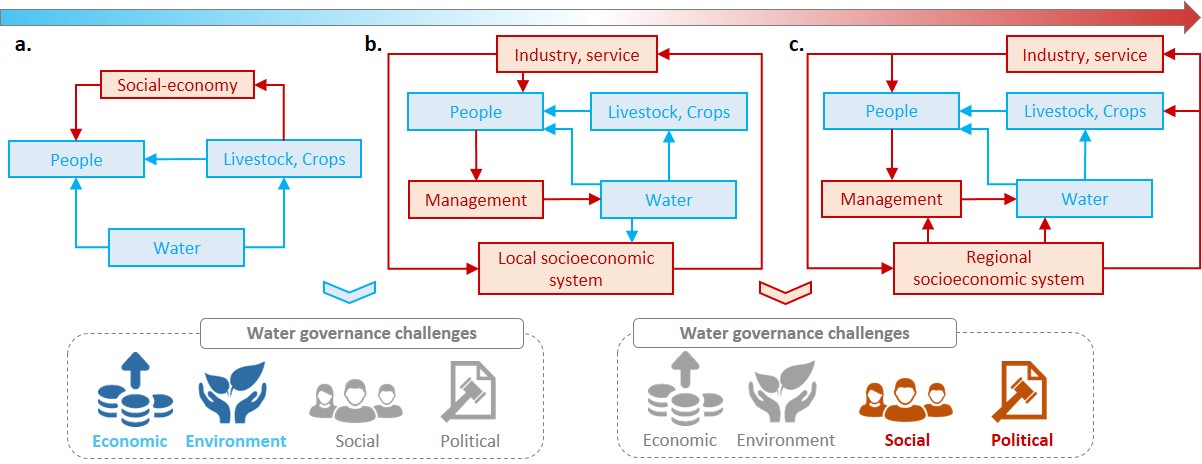
\includegraphics[width=\linewidth]{../../figures/main/transition.jpg}
	\caption{
		\textbf{Transition framework of water utilization.} Blue pathways dominated by natural water loop while red ones dominated by socio-economic loops. 
		\textbf{A. Natural phase:} As an indispensable provisioning resource, the main functions of water resource is to support crop, livestocks and human-beings, which are the basic ecological services.
		\textbf{B. Local phase:} With local socio-economic systems developing, industry and services (also known as the secondary and the tertiary industry) calling for further water consumptions. What's more, better organized socio-economic system and developed technology gives humans abilities in better managing water resources, with intensive intervention in the natural water cycle. 
		\textbf{C. Regional phase:} With further developed and economically efficient industries and services, trade-off between whose water demands with provisional water demands becomes prominent. Rather than determined by local socio-economic systems, water withdrawals and management act as considerations within the entire basin more, therefore. 
	}
	\label{fig:summary}
\end{figure*}

% 上述过渡过程与稳态转换的关联可能是普遍的
The links between the above transition process and the regime shifts of water utilization may be pervasive as socio-economic processes are gradually dominating human-water systems in most river basins.
% 因此,我们在总结黄河流域变化过程的基础上,进一步概念化了水资源利用制度的过渡框架。
As such, we summarized a transition framework, which conceptualizes a general trajectory towards regional socio-economic dominating water utilization stage by stage.
% 水资源利用制度包括压力、倾向性、格局三个重要因素,三个指标在过渡框架中随着不断变化。
In the framework, provisioning water utilization (agriculture, domestic or livestock) are dominated at the primal phase and social processes take over dominating with growths of industry and services in the followed phases, with coordinated considerations of water utilization over the whole basin (Figure~\ref{fig:summary}).

Three dimensions of water utilization are various throughout the transition. 
% 水资源压力
Firstly, while stresses on water resources increases when economic expansion boosting water demands, socio-economic progress can respond to resource scarcity by better management or efficiency. Water resources were becoming more scarce in the YRB from P1 to P3 (\textit{SI Appendix} Fig. S3). However, water utilization stresses changes a lot rather than always increasing, because constructions of reservoir and the increased water use efficiency were all played roles (Figure~\ref{fig:Causes}). Since the scarcity of water resources is directly perceptible and sensitive for utilization, its stresses on societies is one of the most striking drivers to regime shifts within human-water systems \cite{qinFlexibilityIntensityGlobal2019}.
% 水资源倾向性
Secondly, the non-provisioning part of water demands growths with secondary and tertiary industries developing, leading priority of water utilization continually tilted to the socio-economic part. As original region of Ancient Chinese Civilization, the Yellow River Basin used to be dominated by agricultural but converted to an energy industry zone now \cite{WillEnergyBases}. 
As a result, saving water consumption in agriculture and making concessions for industry and energy is widely recognized as solutions for the competing \cite{xiangWillEnergyIndustry2016,bebbWaterRightsTransfers2011}. Anyhow, this changes of priority reflect a truth that growing socio-economic parts are responding to scarcity of water resources and contributing to regime shifts.
% 水资源格局
Last, with tighter socio-economic links and comparative advantages between regions and sectors, the geographic scope of water resource supply and demand allocation is expanding, leading to changing configurations of water utilization. In the Yellow River Basin, the gap of water consumptions between regions and sectors are narrowing, as the result of a carefully designed configuration.
% \cite{wangThirtyYearsYellow2018}. 
% However, the configuration of water utilization is determined on the basis of regional and sectoral economic contexts and developing trajectories 
%\cite{wangThirtyYearsYellow2018}. 
% The changes in water utilization configurations along with regime shifts, therefore, are the outcomes of feedbacks within complex human-water systems.

% 综上所述
By combining the above three dimensions, these changes gradually transformed water utilization regimes in a ``natural phase'' (Figure~\ref{fig:summary}A) to one in local or regional phase (Figure~\ref{fig:summary}B and Figure~\ref{fig:summary}C), with socio-economic processes dominated step by step. In addition to the YRB, human-water relations in major river basins around the world can be explained by the framework. 
For examples, Indus River, Mississippi River, and Danube River, whose water utilizations have all gone through a relatively natural regime, rapid developments and integrated management regimes. 
\cite{bestAnthropogenicStressesWorld2019,cummingResilienceBigRiver2011}. 
In summary, some similar pattern of water utilization can be revealed by the transition framework with basins development.

\section*{Dilemmas and future directions}
% 对于可持续科学,认识这种稳态的变化很重要
% For sustainability scientists, recognizing that different regimes of water utilization regarding different water utilization regimes has important implications for social development and river basin management.
% 不同的流域位于过渡的不同阶段,面临的问题也存在区别,主要包括资源陷阱和结构陷阱两类。
% At different transition phases, however, basins may face to various development dilemmas in water utilization, leading an unsustainable trajectory. 
% % 资源陷阱和失配,导致崩溃
% Like social-ecological systems and other complex systems, coupled human-water system may collapse under the stresses reached the tipping point or structural mismatches 
% \cite{reyersSocialEcologicalSystemsInsights2018,cummingQuantifyingSocialEcologicalScale2020,wangCOSUSTMs0530Review}. 
% % 转型应对陷阱
% A number of studies have identified transformation as an important way out of these unsustainable trajectories, and different types of transformation are required according to dominating regimes and dilemmas of \cite{scoonesTransformationsSustainabilityCombining2020a,steffenTrajectoriesEarthSystem2018}. 
% % 我们的框架有助于理解和识别
Not only the index helps to identify regime shifts of water utilization, our transition framework also helps in predicting possible dilemmas with the development of society.
% 世界各大流域面临的问题。资源开发早期容易陷入资源陷阱;流域发展后期容易陷入结构陷阱。
According to cases all around the world, big river basins often face resource dilemmas after resources-dependent developments, while highly developed ones need to resolve structural problems more often (\textit{SI Appendix} Fig. S11).
% 黄河流域的发展过程,资源开发P2阶段陷入了资源陷阱(表现形式 xxx)。
After the successive exploitation of agriculture, industry and services (refers from natural phase to a local phase in the framework, Figure~\ref{fig:summary}), it is easy for basins to get into a resource dilemma.
% 后来摆脱了资源陷阱(表现形式 xxx)。
As an example, the YRB proposed a clear transformation towards integrated basin management to get rid of the severe resource dilemma, with several management practices. 
% 一段有关87分水方案的介绍
The most important of these is the “87 Water Allocation Scheme”, which adopts a top-down approach in allocating water resources to all regions and sectors. 
%\cite{wangThirtyYearsYellow2018}. 
Since then, the scheme has been revised and refined, and a comprehensive water resources utilization system has gradually formed. 
% \cite{wangThirtyYearsYellow2018}. 
These integrated management practices made the utilization of water resources into a regime of unified scheduling since the P3 in the Yellow River Basin, to escape from the resource dilemma. 
% 资源困局可能普遍存在
Accelerated development has been followed by severe water scarcity and a series of ecological problems, similar dilemmas are pervasive in basins highly dependent on water resources, where in need of moving towards integrated governance as well 
\cite{bestAnthropogenicStressesWorld2019,cummingResilienceBigRiver2011,unep-dhiTransboundaryRiverBasins2016}.
% 通过协同治理来摆脱困局也普遍存在

% 此外,即使发展极大提升了用水效率,黄河流域的困境也并没能完全解决。
In addition, further dilemmas occurred as basins developments tighter interlinked to the ecosystems after integrated management and move to a regional phase (refers from a local phase to a regional phase in the framework, Figure~\ref{fig:summary}).
% 展望:未来还可能陷入结构陷阱,(表现形式:用水效率悖论的同时,倾向性停滞,灵活性进一步降低,)
% Therefore, basins still in need of further transformations according to changes within the transition cycle of water utilization. 
Firstly, significant improvement in agricultural irrigation efficiency has been accompanied by re-expansion in irrigated area, resulting in a usually unabated trend of water resources stress which is known as paradox of efficiency \cite{graftonParadoxIrrigationEfficiency2018}. 
Secondly, the changing priority between non-provisioning (i.e. industry or services) and provisioning (i.e. domestic and irrigation water use) may lead the water utilization more inflexible and damage to resilience of the basin \cite{qinFlexibilityIntensityGlobal2019}.
Take the YRB as an example again, after getting rid of the resource dilemma, the stresses on water resources were still growing, while inflexible water use (domestic and thermal uses) growth most strikingly (supplementary Fig. S4). 
% 这可能对全球的流域都是一个警示,因为
It can be a warning to river basins around the world in comprehensive developments, since these may lead to a reduction in resilience of basins and leave highly coupled human-water systems facing greater vulnerability to collapse --as a structural dilemma \cite{cummingResilienceBigRiver2011}. 

% 下一步:可以通过统一调控,调整格局来调整结构,突破结构陷阱。
% 总结:整个流域需进一步转型与适应,以实现高质量发展。
Taken together, based on the identification of current phases and development dilemmas by the transition framework, further transformative governance is still needed to achieve a high-quality sustainable development of the basin, because development is not a panacea for every dilemma \cite{scoonesTransformationsSustainabilityCombining2020a}.


%tag 研究方法
\matmethods{
Here, we constructed the Integrated Water Resources Utilization (IWRU) Index which consists of three dimensions and identified the changes periods of the index over time by change points detection. 
Each dimension is reflected by an independent indicator after normalization, and water utilization regime were characterized by combination of impacts of each dimension in periods.
In addition, the contribution to changes of IWRU index along with each main indicators were decomposed and calculated separately for each regime (i.e. period). 
	
	\subsection*{Integrated Water Resources Utilization (IWRU) Index}
	% 我们认为水资源利用制度,与水资源利用的三个维度紧密相关:
	Water resources utilization system is closely related to the social developments in three dimensions below (see \textit{SI Appendix} Methods S4 for details):
	
	% - 社会的发展通常伴随着用水向社会经济系统倾斜,用水方式优先向收益更高的非供给性方式倾斜:
	\begin{itemize}
		\item Social development is usually accompanied by a change of priority in water use towards social and economic systems because of higher returns:
		$$ Dev. \propto P $$
		% - 社会发展通常伴随着更具结构性的水资源配置,如区域部门之间的分工合作,以及区域的统筹配置:
		\item Social development usually lead to more complex structure in configuration of water resources, which is a result of division and cooperation between regions and sectors for developing:
		$$ Dev \propto A $$ 
		% - 可持续的社会发展应该通过技术手段有效缓解发展过程中产生的水资源压力,才能实现可持续发展:
		\item Further social development can only be achieved by effectively alleviating the water resource stresses generated in the process of development through technological means:
		$$ Dev \propto S^{-1} $$
	\end{itemize}
	
	% 将三者合一起,即:
	We combine the above three dimensions for an integrated index, remaining their positive or negative relationship with social development: 
	$$ Dev. \propto P*A*S^{-1} $$

	% 在上述假设的基础上,我们要构建流域综合耦合指数(Integrated Water Resources Utilization, IWRU),使 IWRU 有效表征与用水相关的三个维度。首先为每个维度选择一个合适的指示因子(indicator, $I_x$, 其中$x=P, C or S$)。将上式进行自然对数转换,从而让三个维度之间变成加减关系:
	To effectively represent the three dimensions, we select an appropriate indicator ($I_x$, $x=P$, $C$ or $S$ corresponding to Priority, Configuration and Stress respectively) for each dimension. Then, the above equation is transformed into a natural logarithm to facilitate calculation:

	$$ Dev. \propto ln(I_P) + ln(I_A) - ln(I_S) $$

	Assuming they have equal weights, the Integrated Water Resources Utilization (IWRU) Index:

	$$ IWRU = I'_A + I'_P - I'_S $$

	where $I'_x$ is a normalization of log-transformed indicator $I_x$ for a certain dimension:

	$$ I'_x = normalize(ln(I_x)) $$
	
	\subsubsection*{Normalization}
	In fact, we have tested different normalization methods and it makes no difference in change points detection (see \textit{SI Appendix} Methods S5. Sensitivity analysis). In this study, finally, we performed min-max normalization as the formulation below:

	$$ normalize(X) = (X - X_{min}) / (X_{max} - X_{min}) $$

	\subsubsection*{Indicator of Stress}
	We refer to the scarcity-flexibility-variability (SFV) water stress index proposed in Qin et al., 2019 to evaluate water stress ($SFV_i$) as the indicator in a certain region $i$ \cite{qinFlexibilityIntensityGlobal2019}. This metric takes into account management measures (such as the construction of reservoirs) and the impact of changes in the industrial structure of water use on the evaluation of water scarcity (see \textit{SI Appendix} Methods S4 for details). For the whole YRB, indicator of stress $I_S$ is the average stress of all regions' SFV-index: 

	$$ I_S = \frac{1}{4} * \sum_{i=1}^4 SFV_{i} $$
	
	Where $SFV_i$ is the SFV-index for region $i$, and $i=1$ to $4$ refers SR, UR, MR, and DR (see \textit{SI Appendix} Methods S1 Definition of study area).

	\subsubsection*{Indicator of priority}
	To priority $I_P$, we use Non-Provisioning Shares (NPS) of water use as an indicator. While provisional water use ($WU_{pro}$) includes domestic, irrigated and livestock water uses, the non-provisioning water use ($WU_{non-pro}$) includes industrial and urban services water uses. Then, we can calculate the non-provisioning shares by:

	$$ NPS_{i} = \frac{WU_{non-pro, i}}{WU_{pro, i} + WU_{non-pro, i}} $$

	Where $i$ refers a certain region, or the whole basin, i.e:

	$I_P$ = $NPS_{basin}$

	\subsubsection*{Indicator of configurations}
	%$CEM$ 指标度量的是水资源配置“不均匀”的程度,类似于信息熵是对“混乱程度”的度量,即参与分配的各个单位之间,分配比例差距越大,则熵越小。
	% 而我们的指标应反映随着社会发展,水资源配置在区域之间更加均衡(比例差距小)、整体满足不同用水部门的发展需求(比例差距减小)、但不同区域存在部门分工(比例差距增大)的趋势。
	To description of configurations $I_C$, we designed an indicator by imitation of information entropy, called Configuration Entropy Metric (CEM), a metric to measure the degree of evenness of water configuration (see \textit{SI Appendix} Methods S4).
	While our indicator $I_C$ should reflect that with the development of society, water resources configuration is more balanced among regions and generally meets the needs of different sectors (means smaller gaps, too), but different regions have a trend of division of labour among various sectors (with larger gaps):

	$$ I_C = \frac{CEM_{r}*CEM_{s}}{CEM_{rs}}$$
	
	where $CEN_{r}$ and $CEN_{s}$ are Configuration Entropy Metric in different regions and different sectors. $CEN_{rs}$ is differences between sectors in a certain region to the whole basin (see \textit{SI Appendix} Methods S4). 

	\subsection*{Change points detection}
		% The method makes no assumptions about the distribution of the data and detects breakpoints based solely on the probability of the data coming from different distributions before and after the breakpoint.

		With no assumptions about the distribution of the data, the Pettitt (1979) approach of changing points detection is commonly applied to detect a single change-point in hydrological series with continuous data \cite{pettittNonParametricApproachChangePoint1979}. 
		It tests the $H0$: The variables follow one or more distributions that have the same location parameter (no change), against the alternative: a change point exists. The non-parametric statistic is defined as:
	
		$$ K_t = max|U_{t, T}|$$

		Where:

		$$ U_{t, T} = \sum_{i=1}^t\sum_{j=t+1}^T sgn(X_i - X_j) $$
	
		The change-point of the series is located at $K_T$, provided that the statistic is significant. We use 0.001 as the threshold  of p-value (see \textit{SI Appendix} Methods S5 for Sensitivity analysis), which means the probability of a statistically significant change-point judgment being valid is more than $99.9\%$.
		Since this method only can return one significant change point, we repeat it Until all significant change points were detected.
	
	% 计算贡献度
	\subsection*{Contribution decomposition}
		We have decomposed the amount of variation in each index at different stages in order to observe the contribution of each influencing factor to them. Use Integrated Water Resources Utilization (IWRU) Index as an example, which influenced by three dimensions' normalized indicator: stress ($I'_S$), priority ($I'_P$) and configuration ($I'_C$). We can calculate their differences between two certain years ($y_2$ and $y_1$, $y_2 > y_1$) by:

		\begin{align*}
			\Delta IWRU &= (I'_{P_{y_2}} + I'_{C_{y_2}} - I'_{S_{y_2}}) - (I'_{P_{y_1}} + I'_{C_{y_1}} - I'_{S_{y_1}}) \\
			&= (I'_{P_{y_2}} - I'_{P_{y_1}}) + (I'_{C_{y_2}} - I'_{C_{y_1}}) + (I'_{S_{y_1}} - I'_{S_{y_2}}) \\
			&= \Delta I'_P + \Delta I'_C + (-\Delta I'_S)
		\end{align*}
		Then, the contribution of dimension $x$ to IWRU's changes can be referred as:

		$$ Contribution_x = \frac{\Delta I'_x}{|\Delta IWRU|} $$

		% Since $Contribution_x$ can be positive or negative, we used an absolute value to evaluate the contribution (in proportion) of a certain dimension in the all three dimensions to the changes:
		% $$  Contribution_x\% = \frac{|\Delta I'_x|}{\sum_x |\Delta I'_x|} $$

		% or just for contributions (in proportion) within a certain year $j$ to the regime:
		% $$ Contribution_{x,j}\% = \frac{|I'_{x, j}|}{|\sum_x I'_{x, j}|} $$

	\subsection*{Datasets}
	% 为了计算 IWRU ,我们需要计算多个指标及子指标,所有使用的数据集都在表中列出,数据的详细介绍可见补充材料。
	In order to calculate IWRU, we need to calculate multiple indicators and sub-indicators. All the datasets used are listed in the \textit{SI Appendix} table S1. A detailed description of the data can be seen in the supplementary materials \textit{SI Appendix} Methods S2.
}

\showmatmethods{} % Display the Materials and Methods section

\acknow{Please include your acknowledgments here, set in a single paragraph. Please do not include any acknowledgments in the Supporting Information, or anywhere else in the manuscript.}

\showacknow{} % Display the acknowledgments section

% Bibliography
\bibliography{my-papers}
	
\end{document}